\ifx\mlbook\undefined
    \documentclass[10pt,a4paper]{ctexbook}
    \providecommand{\pathroot}{../..}

    \usepackage[CJKbookmarks,colorlinks,linkcolor=red]{hyperref}
    \usepackage{geometry}
    \usepackage{amsmath}

    \geometry{left=3.0cm,right=3.0cm,top=2.5cm,bottom=2.5cm}
    \setmainfont{SimSun}
    \XeTeXlinebreaklocale "zh"
    \XeTeXlinebreakskip = 0pt plus 1pt minus 0.1pt

    \begin{document}
    \setlength{\baselineskip}{20pt}
    \title{Logistic回归}
    \author{Donald Cheung\\jianzhang9102@gmail.com}
    \date{Sep 8, 2017}
    \maketitle
    \tableofcontents
\fi

\chapter{Logistic回归}
\section{Logistic Regression}
这一章用来介绍常用的线性模型,主要包括:多元线性回归、Logistic回归(LR)。

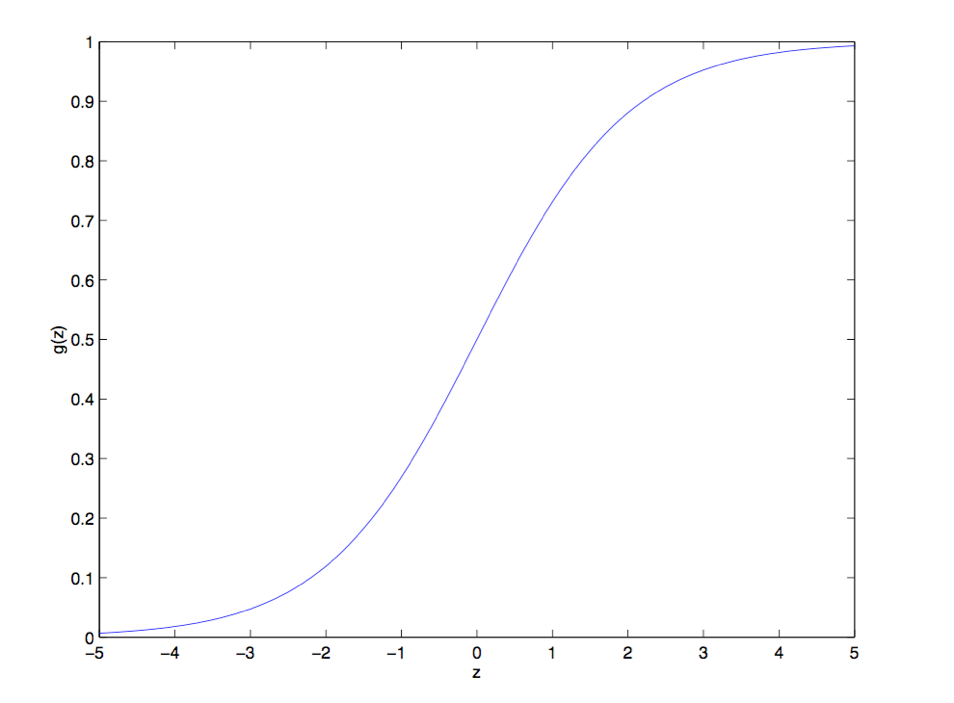
\includegraphics[height=7cm]{\pathroot/theory/lr/images/sigmoid.png}

\section{Logistic回归}
这一章用来介绍常用的线性模型,主要包括:多元线性回归、Logistic回归(LR)。

\subsection{mnist数据集简介}


%$\left(
%  \begin{array}{cccccccccccccccccccccccccccc}
%        0 & 0 & 0 & 0 & 0 & 0 & 0 & 0 & 0 & 0 & 0 & 0 & 0 & 0 & 0 & 0 & 0 & 0 & 0 & 0 & 0 & 0 & 0 & 0 & 0 & 0 & 0 & 0\\
%        0 & 0 & 0 & 0 & 0 & 0 & 0 & 0 & 0 & 0 & 0 & 0 & 0 & 0 & 0 & 0 & 0 & 0 & 0 & 0 & 0 & 0 & 0 & 0 & 0 & 0 & 0 & 0\\
%        0 & 0 & 0 & 0 & 0 & 0 & 0 & 0 & 0 & 0 & 0 & 0 & 0 & 0 & 0 & 0 & 0 & 0 & 0 & 0 & 0 & 0 & 0 & 0 & 0 & 0 & 0 & 0\\
%        0 & 0 & 0 & 0 & 0 & 0 & 0 & 0 & 0 & 0 & 0 & 0 & 0 & 0 & 0 & 0 & 0 & 0 & 0 & 0 & 0 & 0 & 0 & 0 & 0 & 0 & 0 & 0\\
%        0 & 0 & 0 & 0 & 0 & 0 & 0 & 0 & 0 & 0 & 0 & 0 & 0 & 0 & 0 & 0 & 0 & 0 & 0 & 0 & 0 & 0 & 0 & 0 & 0 & 0 & 0 & 0\\
%        0 & 0 & 0 & 0 & 0 & 0 & 0 & 0 & 0 & 0 & 0 & 0 & 3 & 18 & 18 & 18 & 126 & 136 & 175 & 26 & 166 & 255 & 247 & 127 & 0 & 0 & 0 & 0\\
%        0 & 0 & 0 & 0 & 0 & 0 & 0 & 0 & 30 & 36 & 94 & 154 & 170 & 253 & 253 & 253 & 253 & 253 & 225 & 172 & 253 & 242 & 195 & 64 & 0 & 0 & 0 & 0\\
%        0 & 0 & 0 & 0 & 0 & 0 & 0 & 49 & 238 & 253 & 253 & 253 & 253 & 253 & 253 & 253 & 253 & 251 & 93 & 82 & 82 & 56 & 39 & 0 & 0 & 0 & 0 & 0\\
%        0 & 0 & 0 & 0 & 0 & 0 & 0 & 18 & 219 & 253 & 253 & 253 & 253 & 253 & 198 & 182 & 247 & 241 & 0 & 0 & 0 & 0 & 0 & 0 & 0 & 0 & 0 & 0\\
%        0 & 0 & 0 & 0 & 0 & 0 & 0 & 0 & 80 & 156 & 107 & 253 & 253 & 205 & 11 & 0 & 43 & 154 & 0 & 0 & 0 & 0 & 0 & 0 & 0 & 0 & 0 & 0\\
%        0 & 0 & 0 & 0 & 0 & 0 & 0 & 0 & 0 & 14 & 1 & 154 & 253 & 90 & 0 & 0 & 0 & 0 & 0 & 0 & 0 & 0 & 0 & 0 & 0 & 0 & 0 & 0\\
%        0 & 0 & 0 & 0 & 0 & 0 & 0 & 0 & 0 & 0 & 0 & 139 & 253 & 190 & 2 & 0 & 0 & 0 & 0 & 0 & 0 & 0 & 0 & 0 & 0 & 0 & 0 & 0\\
%        0 & 0 & 0 & 0 & 0 & 0 & 0 & 0 & 0 & 0 & 0 & 11 & 190 & 253 & 70 & 0 & 0 & 0 & 0 & 0 & 0 & 0 & 0 & 0 & 0 & 0 & 0 & 0\\
%        0 & 0 & 0 & 0 & 0 & 0 & 0 & 0 & 0 & 0 & 0 & 0 & 35 & 241 & 225 & 160 & 108 & 1 & 0 & 0 & 0 & 0 & 0 & 0 & 0 & 0 & 0 & 0\\
%        0 & 0 & 0 & 0 & 0 & 0 & 0 & 0 & 0 & 0 & 0 & 0 & 0 & 81 & 240 & 253 & 253 & 119 & 25 & 0 & 0 & 0 & 0 & 0 & 0 & 0 & 0 & 0\\
%        0 & 0 & 0 & 0 & 0 & 0 & 0 & 0 & 0 & 0 & 0 & 0 & 0 & 0 & 45 & 186 & 253 & 253 & 150 & 27 & 0 & 0 & 0 & 0 & 0 & 0 & 0 & 0\\
%        0 & 0 & 0 & 0 & 0 & 0 & 0 & 0 & 0 & 0 & 0 & 0 & 0 & 0 & 0 & 16 & 93 & 252 & 253 & 187 & 0 & 0 & 0 & 0 & 0 & 0 & 0 & 0\\
%        0 & 0 & 0 & 0 & 0 & 0 & 0 & 0 & 0 & 0 & 0 & 0 & 0 & 0 & 0 & 0 & 0 & 249 & 253 & 249 & 64 & 0 & 0 & 0 & 0 & 0 & 0 & 0\\
%        0 & 0 & 0 & 0 & 0 & 0 & 0 & 0 & 0 & 0 & 0 & 0 & 0 & 0 & 46 & 130 & 183 & 253 & 253 & 207 & 2 & 0 & 0 & 0 & 0 & 0 & 0 & 0\\
%        0 & 0 & 0 & 0 & 0 & 0 & 0 & 0 & 0 & 0 & 0 & 0 & 39 & 148 & 229 & 253 & 253 & 253 & 250 & 182 & 0 & 0 & 0 & 0 & 0 & 0 & 0 & 0\\
%        0 & 0 & 0 & 0 & 0 & 0 & 0 & 0 & 0 & 0 & 24 & 114 & 221 & 253 & 253 & 253 & 253 & 201 & 78 & 0 & 0 & 0 & 0 & 0 & 0 & 0 & 0 & 0\\
%        0 & 0 & 0 & 0 & 0 & 0 & 0 & 0 & 23 & 66 & 213 & 253 & 253 & 253 & 253 & 198 & 81 & 2 & 0 & 0 & 0 & 0 & 0 & 0 & 0 & 0 & 0 & 0\\
%        0 & 0 & 0 & 0 & 0 & 0 & 18 & 171 & 219 & 253 & 253 & 253 & 253 & 195 & 80 & 9 & 0 & 0 & 0 & 0 & 0 & 0 & 0 & 0 & 0 & 0 & 0 & 0\\
%        0 & 0 & 0 & 0 & 55 & 172 & 226 & 253 & 253 & 253 & 253 & 244 & 133 & 11 & 0 & 0 & 0 & 0 & 0 & 0 & 0 & 0 & 0 & 0 & 0 & 0 & 0 & 0\\
%        0 & 0 & 0 & 0 & 136 & 253 & 253 & 253 & 212 & 135 & 132 & 16 & 0 & 0 & 0 & 0 & 0 & 0 & 0 & 0 & 0 & 0 & 0 & 0 & 0 & 0 & 0 & 0\\
%        0 & 0 & 0 & 0 & 0 & 0 & 0 & 0 & 0 & 0 & 0 & 0 & 0 & 0 & 0 & 0 & 0 & 0 & 0 & 0 & 0 & 0 & 0 & 0 & 0 & 0 & 0 & 0\\
%        0 & 0 & 0 & 0 & 0 & 0 & 0 & 0 & 0 & 0 & 0 & 0 & 0 & 0 & 0 & 0 & 0 & 0 & 0 & 0 & 0 & 0 & 0 & 0 & 0 & 0 & 0 & 0\\
%        0 & 0 & 0 & 0 & 0 & 0 & 0 & 0 & 0 & 0 & 0 & 0 & 0 & 0 & 0 & 0 & 0 & 0 & 0 & 0 & 0 & 0 & 0 & 0 & 0 & 0 & 0 & 0
%    \end{array}
%\right)$

\subsection{Logistic Regression}

\begin{itemize}
\item logistic函数/sigmoid函数: $h_{\theta}(x)=g({\theta}^Tx)={\frac {1}{1+e^{-\theta^Tx}}}$ 
\item 函数可导:
$g'(z)={\frac {d}{dz}}{\frac {1}{1+e^{-\theta^Tx}}}=\lim_{{\Delta x}\to 0}{\frac {f(x+{\Delta x})-f(x)}{\Delta x}}$
\end{itemize}

\begin{itemize}
\item 对于一个二分类问题,可假设$h_{\theta}(x)$为其中一类的概率,即:
\subitem $P(y=1|x;\theta)=h_{\theta}(x)$
\subitem $P(y=0|x;\theta)=1-h_{\theta}(x)$
\item 更简洁的形式: $P(y|x;\theta)={h_{\theta}(x)}^y(1-h_{\theta}(x))^{1-y}$
\item 假设$m$个训练样本独立,则样本集在参数${\theta}$给定下,出现的概率为:

\item 我们希望最大化概率$L({\theta})$,也即最大化log似然值:

\item 最大化一个目标值,可采用梯度上升法,沿着梯度方向不断迭代。梯度求解如下:

\item 随机梯度下降法求解:
\subitem ${\theta}_{j}:={\theta}_{j}+{\alpha}(y^{(i)}-h_{\theta}(x^{(i)}))x_{j}^{(i)}$

\item 思考:
\subitem 如果引入$L1$正则、$L2$正则,那么梯度又该怎么求解呢?
\subitem LR的梯度求解公式与线性回归的梯度求解公式看起来一样,有区别么?

\item L1:$cost(w)={\frac {1}{2m}}\left\|{Xw-y}\right\|^{2}+\lambda\|w\|_{1}$
,等价于
    $\min\limits_{w}{\frac {1}{2m}}\left\|{Xw-y}\right\|^{2}, s.t. \left\|w\right\|_{1}\le{C}$

\item L2:$cost(w)={\frac {1}{2m}}\left\|{Xw-y}\right\|^{2}+{\frac {\lambda}{2}}\|w\|_{2}^{2}$
,等价于
    $\min\limits_{w}{\frac {1}{2m}}\left\|{Xw-y}\right\|^{2}, s.t. \left\|w\right\|_{2}^{2}\le{C}$

\item 常用分类器的评价指标有:准确率(precision)、召回率(recall)、F值、正确率(accuracy)等
\end{itemize}

\begin{itemize}

\item 考虑ROC曲线图中的四个点。
    \subitem(1)第一个点(0,1),FPR=0, TPR=1,即FN=0,并且FP=0。
        \subsubitem 特点:正确分类所有的样本。
    \subitem(2)第二个点(1,0),FPR=1,TPR=0。
        \subsubitem 特点:成功错分了所有的样例。
    \subitem(3)第三个点(0,0),FPR=TPR=0,即FP=TP=0,
        \subsubitem 特点:分类器预测所有的样本都为负样本。
    \subitem(4)第四个点(1,1),分类器预测所有的样本都为正样本。
\item 结论:ROC曲线越接近左上角,该分类器的性能越好。
\item 考虑ROC曲线图中的虚线$y=x$上的点。这条对角线上的点表示的是一个采用随机猜测策略的分类器的结果。

\item ROC曲线的画法:对一个特定的测试数据集合,对分类模型输出的概率值设置不同的阈值,从而得到一组(FPR,TPR)点,以此连接这些点即可得到ROC曲线。
\item AUC(Area Under Curve):ROC曲线下的面积。
\item AUC值等于一个随机选择的正样本的预测值高于一个随机选择的负样本的概率。
\item ROC曲线的优点:当测试集中的正负样本的分布变化的时候,ROC曲线能够保持不变。

\item 在右图中,(a)和(c)为ROC曲线,(b)和(d)为\\
Precision-Recall曲线。(a)和(b)展示的是\\
分类其在原始测试集(正负样本分布平衡)\\
的结果,(c)和(d)是将测试集中负样本的数\\
量增加到原来的10倍后, 分类器的结果。可\\
以明显的看出,ROC曲线基本保持原貌,\\
而Precision-Recall曲线则变化较大。

\item 基本思路:将多分类任务拆若干个二分类任务。学习时分别训练多个分类器,测试时对这多个分类器的预测结果进行集成以获得最终的多分类结果
\item 一对一(OvO) 
    \subitem 以$C_{i}$与$C_{j}$的数据作为正反例训练一个分类器,共训练${\frac {N(N-1)}{2}}$个分类器
    \subitem 预测时将样本提交给所有分类器,获取${\frac {N(N-1)}{2}}$个结果,最终结果通过投票产生
\item 一对多(OvR)
    \subitem 以$C_{i}$数据为正例,其余类别数据为负例,训练$N$个分类器
\item 其他:如多对多(MvM)策略的ECOC编码
\end{itemize}

\section{Softmax Regression}
这一章用来介绍常用的线性模型,主要包括:多元线性回归、Logistic回归(LR)。

\subsection{Softmax Regression}

\begin{itemize}
\item 简介:为LR在多分类上的推广。与LR一样,同属于广义线性模型(Generalized Linear Model)。
\item $P(y=i|x;{\theta})={\frac {e^{{\theta}_{i}^{T}x}}{\sum_{j=1}^{K}{e^{{\theta}_{j}^{T}x}}}}$
\item 同样,考虑使得对数似然最大,则系统损失函数为:\\
    $\ell(\theta)=-{\frac {1}{m}}\left[\sum\limits_{i=1}^{m}{\sum\limits_{j=1}^{K}{1\{y^{(i)}=j\}\log{\frac{e^{{\theta}_{j}^{T}{x^{(i)}}}}{\sum_{l=1}^{K}{e^{\theta_{l}^{T}x^{(i)}}}}}}}\right]$
\item 加入正则项:\\
    $\ell(\theta)=-{\frac {1}{m}}\left[\sum\limits_{i=1}^{m}{\sum\limits_{j=1}^{K}{1\{y^{(i)}=j\}\log{\frac{e^{{\theta}_{j}^{T}{x^{(i)}}}}{\sum_{l=1}^{K}{e^{\theta_{l}^{T}x^{(i)}}}}}}}\right]+
    {\frac {\lambda}{2}{\sum\limits_{i=1}^{K}{\sum\limits_{j=0}^{n}{\theta_{ij}^{2}}}}}$

\item 考虑一个样本$(x,y)$,有$\ell(x,\hat{y})=-\sum\limits_{j=1}^{K}{1\{y=j\}\ln{\hat{y}_{j}}}$,令$a_{j}={\theta_{j}^{T}x}$,有
\begin{align*}
{\frac {\partial \ell(x,\hat{y})}{a_{j}}}&=\sum\limits_{i=1}^{K}{{\frac {\partial \ell(x,\hat{y})}{\partial \hat{y}_{i}}}{\frac {\partial \hat{y}_{i}}{\partial a_{j}}}}\\
                                         &=-\sum\limits_{i=1}^{K}{
                                                {\frac {1\{y=i\}}{\hat{y}_{i}}}
                                                {\frac {\partial \frac {e^{a_{i}}}{\sum_{l=1}^{K}{e^{a_{l}}}}}{\partial a_{j}}}}\\
                                         &=-\sum\limits_{i=1}^{K}{
                                                {\frac {1\{y=i\}}{\hat{y}_{i}}}
                                                {\frac {
                                                            e^{a_{i}} \cdot 1\{i=j\} \cdot {\left({\sum_{l=1}^{K}{e^{a_{l}}}}\right)}
                                                            -e^{a_{i}} \cdot e^{a_{j}}
                                                        }
                                                       {\left({\sum_{l=1}^{K}{e^{a_{l}}}}\right)^{2}}
                                                    }}\\
                                         &=\sum\limits_{i=1}^{K}{
                                                {\frac {1\{y=i\}}{\hat{y}_{i}}}
                                                {\frac {e^{a_{i}} \cdot e^{a_{j}}}
                                                       {\left({\sum_{l=1}^{K}{e^{a_{l}}}}\right)^{2}}
                                                    }}
                                            -\sum\limits_{i=1}^{K}{
                                                {\frac {1\{y=i\}}{\hat{y}_{i}}}
                                                {\frac {e^{a_{i}} \cdot 1\{i=j\} \cdot {\left({\sum_{l=1}^{K}{e^{a_{l}}}}\right)}}
                                                       {\left({\sum_{l=1}^{K}{e^{a_{l}}}}\right)^{2}}
                                                    }}\\
                                         &=\sum\limits_{i=1}^{K}{{\frac {1\{y=i\}}{\hat{y}_{i}}}{\hat{y}_{i}}{\hat{y}_{j}}}
                                            -\sum\limits_{i=1}^{K}{{\frac {1\{y=i\}}{\hat{y}_{i}}}{\hat{y}_{i}} \cdot 1\{i=j\}}\\
                                         &={\hat{y}_{j}}-\sum\limits_{i=1}^{K}{{1\{y=i\}}} \cdot 1\{i=j\}\\
                                         &={\hat{y}_{j}}-{1\{y=j\}} \\
\end{align*}


\item 如果待分的类别互斥,使用softmax
\item 如果类别有交叉,则使用LR进行投票分类
\item 例如
    \subitem 有四个类别的音乐,分别为:古典音乐、乡村音乐、摇滚乐和爵士乐
    \subitem 有四个类别如下:人声音乐、舞曲、影视原声、流行歌曲


\item 实际工程中,LR很少使用连续特征。一般将连续特征离散化成多个取值为0/1的离散特征。
\subitem 0. 离散特征的增加和减少都很容易,易于模型的快速迭代;
\subitem 1. 稀疏向量内积乘法运算速度快,计算结果方便存储,容易扩展;
\subitem 2. 离散化后的特征对异常数据有很强的鲁棒性;
\subitem 3. 逻辑回归属于广义线性模型,表达能力受限;离散化相当于为模型引入了非线性,提升模型表达能力;
\subitem 4. 离散化后可以进行特征交叉,由$M+N$个变量变为$M*N$个变量,进一步引入非线性,提升表达能力;
\subitem 5. 特征离散化后,模型会更稳定;
\subitem 6. 特征离散化以后,起到了简化了逻辑回归模型的作用,降低了模型过拟合的风险。

\end{itemize}




\begin{itemize}
\item 监督学习:利用一组已知类别的样本调整分类器的参数,\\使其达到所要求性能的过程
\item 一些符号定义:

$x^{(i)}$:指数据集中的第$i$个样本的特征类数据。

$y^{(i)}$:指数据集中的第$i$个样本的目标值。

$\left(x^{(i)},y^{(i)}\right)$:表示一个样本实例。

$\left\{\left(x^{(i)},y^{(i)}\right), i=1,...,N\right\}$:表示一个数据集。
\\例如,对于手写体识别来说,图片的像素表示即为特征$x$,图片表示的数字即为目标值$y$。

\end{itemize}

对于红酒问题,
\begin{itemize}
\item 问题分析:
\\(1) 共有11个特征,可表示为11个变量:$x^{(i)}_1,x^{(i)}_2,...,x^{(i)}_{11}$。
\\(2) 目标只有一个评分,可表示为:$y^{(i)}$
\\(3) 问题可表示为优化问题:$argmin_{w}\sum_{i=1}^{N}(w_0 + w_1*x^{(i)}_1 + w_2*x^{(i)}_2 + w_{11}*x^{(i)}_{11} - y^{(i)})^2$

\item 用向量表示更加简洁:
\\(1) 特征表示为:$x^{(i)}=\left(\begin{array}{ccc}x^{(i)}_0,x^{(i)}_1,...,x^{(i)}_{11}\end{array}\right)^T$,其中$x^{(i)}_0=1$
\\(2) 权重系数表示为:$w=\left(\begin{array}{ccc}w_0,w_1,...,w_{11}\end{array}\right)^T$
\\(3) 问题表示为:$argmin_{w} \sum_{i=1}^{N}(w^Tx^{(i)}-y^{(i)})^2$

\end{itemize}

\begin{equation}
  s_{kk'}=
  \left(
  \begin{array}{ccc}
          h_{1k} &
          \cdots &
          h_{nk}
  \end{array}
  \right)
  \left(
  \begin{array}{ccc}
          \bar{q}_{11} & \cdots & \bar{q}_{12}\\
          \vdots & \ddots & \vdots\\
          \bar{q}_{n1} & \cdots & \bar{q}_{n2}
  \end{array}
  \right)
  \left(
  \begin{array}{c}
          h_{1k'} \\
          \vdots \\
          h_{nk'}
 \end{array}
 \right)
\end{equation}


%\\$x=\begin{matrix} 0 & 1 \end{matrix}$

\subsubsection{Linear Regression}
\begin{itemize}

\item 给定一份数据集$\left\{x_0^{(i)},x_1^{(i)},...,x_m^{(i)},y^{(i)}\right\}_{i=0}^{N-1}$,线性回归假设目标值$y^{(i)}$与特征$x^{(i)}$之间为线性关系,即:$$y^{(i)}=w_0x_0^{(i)}+w_1x_1^{(i)}+...+w_mx_m^{(i)}$$

\item 现实世界不存在完美线性相关的关系,总会有各\\
种各样的偏差存在。由大数定理,可假设真实值\\
总在理论值附近波动,误差符合高斯分布, 即:\\
$y^{(i)}=w_0x_0^{(i)}+w_1x_1^{(i)}+...+w_mx_m^{(i)}+\varepsilon^{(i)}$\\
其中,$\varepsilon^{(i)}\sim{\mathcal{N}}(0, \sigma^{2})$
%其中,$\varepsilon\sim{\mathcal{N}}(\mu, \sigma^{2})$

\item 假设训练集中一共有$N$个样本:

$X=\left(
\begin{array}{c}
        {(x^{(0)})}^T \\
        {(x^{(1)})}^T \\
        \vdots \\
        {(x^{(N-1)})}^T \\
\end{array}
\right)=\left(
\begin{array}{ccc}
        x_0^{(0)} & \cdots & x_m^{(0)} \\
        x_0^{(1)} & \cdots & x_m^{(1)} \\
        \vdots & \ddots & \vdots\\
        x_0^{(N-1)} & \cdots & x_m^{(N-1)}
\end{array}
\right)$
$w=\left(
\begin{array}{c}
        w^{(0)} \\
        w^{(1)} \\
        \vdots \\
        w^{(m)}
\end{array}
\right)$
$y=\left(
\begin{array}{c}
        y^{(0)} \\
        y^{(1)} \\
        \vdots \\
        y^{(N-1)}
\end{array}
\right)$

\item 线性回归的目标就是最小化预估值与真实值的差距,也即所求$w$满足:$$argmin \left\|{Xw-y}\right\|^{2}$$
\item 代数解:$w=(X^{T}X)^{-1}X^{T}y$
\end{itemize}


\begin{itemize}
\item 代数解非常优美:\\
(1) 当$X^{T}X$为满秩矩阵或正定矩阵时,上式有唯一解。\\
(2) 现实任务中往往不是满秩矩阵,即$X^{T}X$不可逆,原因有很多,例如:
    \begin{itemize}
    \item 存在冗余特征,例如特征之间相关
    \item 训练样本少,如特征数甚至超过样本数
    \end{itemize}
此时$w$有多个可行解,需要选择最佳$w$。 \\
(3) 此代数解运算复杂度高,当$n>10000$时开销过大。\\

\end{itemize}

\subparagraph{梯度下降}
介绍梯度下降的原理。
\subsection{理论}

\begin{itemize}
\item 想法:人类在学习的时候,都是渐进式学习,不断从错误中纠正自己的认知,从而越来越优秀。
\item 导数定义:$ {\frac {dy}{dx}}={\frac {df}{dx}}(x)={\frac {d}{dx}}f(x)=f'(x)=\lim_{{\Delta x}\to 0}{\frac {f(x+{\Delta x})-f(x)}{\Delta x}} $\\
有:$f(x+{\Delta x})-f(x)=f'(x){\Delta x}$
\\(1) 如果$f'(x)>0$:
\subitem 当${\Delta x}>0$时,$f(x+{\Delta x})-f(x)=f'(x){\Delta x}>0$;
\subitem 当${\Delta x}<0$时,$f(x+{\Delta x})-f(x)=f'(x){\Delta x}<0$
\\(2) 如果$f'(x)<0$:
\subitem 当${\Delta x}>0$时,$f(x+{\Delta x})-f(x)=f'(x){\Delta x}<0$;
\subitem 当${\Delta x}<0$时,$f(x+{\Delta x})-f(x)=f'(x){\Delta x}>0$
\item 结论:如果使$x$变化的方向与$f'(x)$一致,将会使得$f(x)$增加。
\end{itemize}

\begin{itemize}
\item 梯度:$\nabla f=\left({\frac {\partial f}{\partial x_{1}}},\dots ,{\frac {\partial f}{\partial x_{n}}}\right)$,其中$\left(\nabla f\right)_{i}={\frac {\partial f}{\partial x_{i}}}$
\item 梯度下降算法(Gradient Descent):沿梯度下降的方向求解极小值。
\item 算法过程:
\\(1) 初始化参数为任意值。例如线性回归中的$w$。
\\(2) 求解梯度。例如线性回归中,求解 $\nabla\left(\left\|{Xw-y}\right\|^{2}\right)$。
\\(3) 更新参数。例如线性回归中,更新参数$w$,\\使得$w=w-\alpha\nabla\left(\left\|{Xw-y}\right\|^{2}\right)$,$\alpha$称为学习率。
\\(4) 若达到指定迭代次数或者收敛条件,训练结束。\\否则,继续执行步骤(2)。
\end{itemize}

\begin{itemize}
\item 实际应用中,对梯度下降算法有很多变形或改进。
\item 随机梯度下降(stochastic gradient descent):每遇到
\\一个或者多个但不是整个样本集,就计算梯度,更新参数。
\item 算法过程:
\\(1) 初始化参数为任意值。例如线性回归中的$w$。
\\(2) 对样本集中的每个样本,做如下操作直接完成所有样本\\的遍历:
\subitem(2.1) 求解梯度。例如线性回归中,求解 $\nabla\left(\left\|{Xw-y}\right\|^{2}\right)$。
\subitem(2.2) 更新参数。例如线性回归中,更新参数$w$,使得$w=w-\alpha\nabla\left(\left\|{Xw-y}\right\|^{2}\right)$。
\\(3) 若达到指定迭代次数或者收敛条件,训练结束。否则,继续执行步骤(2)。
\end{itemize}

\begin{itemize}
\item 一个完整的有监督学习的开发流程:
\\(1) 获取数据,对数据做一些清洗、转换等操作。
\\(2) 将数据样本拆分成训练集、验证集和测试集。训练集用来训练模型,验证集用来评估模型效果和调参,测试集则用来评估最终的模型效果。
\\(3) 开发模型或直接使用开发好的模型工具,在训练集上进行训练。
\\(4) 获取训练好的模型,使用验证集评估其效果。如果没有达到预期,需要进一步对模型调参、获取新的特征等操作,直到满足训练效果为止。
\\(5) 使用训练好的模型,在测试集上评估其最终效果。

\item 对于葡萄酒质量预估任务来说,主要有以下过程(只使用白酒的数据):
\\(1) 获取数据集,对数据集做一些预处理操作。
\\(2) 将处理好的数据集分为训练集、验证集和测试集,比例为:0.7:0.2:0.1。
\\(3) 开发线性回归模型。
\\(4) 在训练集上训练线性模型,在验证集上验证模型效果。没有达到预期,需要调参,直到满足训练效果为止。
\\(5) 在测试集中获取最终效果。

\end{itemize}

$x'={\frac {x - x_{min}}{x_{max} - x_{min}}}$

\begin{itemize}
\item 正则项:为有效控制模型参数的复杂度,加入参数复杂度的惩罚项,以使得模型选择更加简单的参数。
\item L1正则:$cost(w)={\frac {1}{2N}}\left\|{Xw-y}\right\|^{2}+\lambda\|w\|_{1}$
\item L2正则:$cost(w)={\frac {1}{2N}}\left\|{Xw-y}\right\|^{2}+{\frac {\lambda}{2}}\|w\|_{2}^{2}$
\\

加入正则项后,梯度:
\item L1正则:$w=w-\alpha (w^{T}x^{(i)}-y^{(i)})x^{(i)} - \alpha\lambda w$
\item L2正则:$w=w-\alpha (w^{T}x^{(i)}-y^{(i)})x^{(i)} - \alpha\lambda sign(w)$
\end{itemize}

\begin{itemize}
\item 优化目标:$cost(w)={\frac {1}{2N}}\left\|{Xw-y}\right\|^{2}$
\item 对于单个样本来说:$cost(w)={\frac {1}{2}}\left({w^{T}x^{(i)}-y^{(i)}}\right)^{2}$
\item 单个样本的梯度为:$\nabla cost(w)=(w^{T}x^{(i)}-y^{(i)})x^{(i)}$
\item 梯度更新:$w=w-\alpha (w^{T}x^{(i)}-y^{(i)})x^{(i)}$
\item 样本特征的取值情况如右图所示
\item 特征归一化: $x'={\frac {x - x_{min}}{x_{max} - x_{min}}}$

\end{itemize}

\subsection{交叉验证{\color{red} TODO}}

交叉验证(Cross Validation),有的时候也称作循环估计(Rotation Estimation),是一种统计学上将数据样本切割成较小子集的实用方法,该理论是由Seymour Geisser提出的。

在模式识别(Pattern Recognition)和机器学习(Machine Learning)的相关研究中,经常会将整个数据集合分成两个部分,分别是训练集合和测试集合。假设X是集合全体,A是全集X的非空真子集,那么非空集合X\textbackslash{A}则是集合A在全集X中的补集。于是可以先在A上面做训练和分析,而集合X\textbackslash{A}则用来做测试和验证。一开始的集合A被称作训练集,而它的补集X\textbackslash{A}被称作验证集或者测试集。这里有一个重要的观点就是:只有训练集才可以使用在模型的训练之中,而测试集必须在模型训练完成之后才被用来评估模型的误差。

\subsubsection{HoldOut检验(Hold-Out Method)}
这个方法是将原始的数据集合X随机分成两个集合A和X\textbackslash{A},其中A作为训练集,X\textbackslash{A}作为测试集。先使用训练集训练模型,然后利用测试集验证模型的效果,记录最后的分类准确率作为Hold-Out下该模型的性能指标。比方说,处理时间序列模型是否准确的时候,把整个数据集合分成前后两部分,前部分占比70\%,后部分占比30\%。前部分来进行时间序列模型的训练,后部分用来测试改时间序列的准确性。其准确性可以用MAE,MAPE之类的统计指标来衡量。综上所述,该方法的好处就是处理起来简单,只需要把原始数据分成两个部分即可。但是从严格意义上来说,Hold-Out检验并不算是交叉检验(Cross Validation),因为该方法没有达到交叉检验的思想,而且最后验证准确性的高低和原始数组的分类有很大的关系,所以该方法得到的结果在某些场景中并不具备特别大的说服力。在Hold-Out检验不够有说服力的情形下,有人提出了交叉验证这一个重要思想。

\textbf{testing中文}
\bf{testing中文}

\subsubsection{交叉检验的常见形式}
假设有一个未知模型有一个或者多个未知的参数,并且有一个训练集。操作的过程就是对该模型的参数进行调整,使得该模型能够最大的反映训练集的特征。如果模型因为训练集过小或者参数不合适而产生过度拟合的情况,测试集的测试效果就可以得到验证。交叉验证是一种能够预测模型拟合性能的有效方法。

\subsubsection{彻底的交叉验证(Exhaustive Cross Validation)}
彻底的交叉验证方法指的是遍历全集X的所有非空真子集A。换句话说也就是把A当作训练集,X\textbackslash{A}是测试集。如果X中有n个元素,那么非空真子集A的选择方法则是$2^{n}-2$,这个方法的时间复杂度是指数级别的。

\begin{itemize}
\item 留P验证(Leave-p-out Cross Validation)
留p验证(LpO CV)指的是使用全集X中的p个元素作为测试集,然后剩下的n-p个元素作为训练集。根据数学上的定理可以得到,p个元素的选择方法有n!/((n-p)!p!)个,其中n!表示n的阶乘。在这个意义下,留p验证的时间复杂度也是非常高的。当p=1的时候,留1验证(Leave-one-out Cross Validation)的复杂度恰好是n。

\item 不彻底的交叉验证(Non-exhaustive Cross Validation)
不彻底的交叉验证不需要考虑全集X的所有划分情况,这种方法是留p验证的一个近似验证算法。

\item k-fold交叉验证(K-fold Cross Validation)
在k-fold交叉验证中,全集X被随机的划分成k个同等大小的集合A1,...,Ak,并且|A1|=...=|Ak|。这里的|Ai|指的是集合Ai的元素个数,也就是集合的势。这个时候需要遍历i从1到k,把X\textbackslash{Ai}当作训练集合,Ai当作测试集合。根据模型的测试统计,可以得到Ai集合中测试错误的结果数量ni。如果全集X的势是n的话,可以得到该模型的错误率是E=(ni求和)/n.
为了提高模型的精确度,可以将k-fold交叉验证的上述步骤重复t次,每一次都是随机划分全集X。在t次测试中,会得到t个模型的错误率E1,...,Et。令e=(Ei求和)/t。这样该模型的错误率就是e。

注释:
一般来说,k=10的情况使用得最多。
当k=2的时候,也就是最简单的k-fold交叉验证,2-fold交叉验证。这个时候X是A1和A2的并集,首先A1当训练集并且A2当测试集,然后A2当训练集并且A1当测试集。2-fold交叉验证的好处就是训练集和测试集的势都非常大,每个数据要么在训练集中,要么在测试集中。
当k=n的时候,也就是n-fold交叉验证。这个时候就是上面所说的留一验证(Leave-one-out Cross Validation)。
\end{itemize}
综上所述,交叉验证(Cross Validation)的好处是可以从有限的数据中获得尽可能多的有效信息,从而可以从多个角度去学习样本,避免陷入局部的极值。在这个过程中,无论是训练样本还是测试样本都得到了尽可能多的学习。

一般模型的选择过程:
在了解了交叉验证的方法之后,可以来介绍一般模型的选择过程。通过采用不同的输入训练样本,来决定机器学习算法中包含的各个参数值,称作模型选择。下面伪代码表示了模型选择的一般流程。在这个算法中,最重要的就是第三个步骤中的误差评价。 
(1)准备候选的q个模型:M1,...,Mq。 
(2)对每个模型M1,...,Mq求解它的学习结果。 
(3)对每个学习结果的误差e1,...,eq进行计算。这里可以使用上面所说的k-fold交叉验证方法。 
(4)选择误差e1,...,eq最小的模型作为最终的模型。









交叉验证是一种用来评价一个统计分析的结果是否可以推广到一个独立的数据集上的技术。主要用于预测,即,想要估计一个预测模型的实际应用中的准确度。它是一种统计学上将数据样本切割成较小子集的实用方法。于是可以先在一个子集上做分析, 而其它子集则用来做后续对此分析的确认及验证。 

交叉验证的理论是由Seymour Geisser所开始的。 它对于防范testing hypotheses suggested by the data是非常重要的,特别是当后续的样本是危险、成本过高或不可能(uncomfortable science)去搜集。

一个交叉验证将样本数据集分成两个互补的子集,一个子集用于训练(分类器或模型)称为训练集(training set);另一个子集用于验证(分类器或模型的)分析的有效性称为测试集(testing set)。利用测试集来测试训练得到的分类器或模型,以此作为分类器或模型的性能指标。

得到高度预测精确度和低的预测误差,是研究的期望。为了减少交叉验证结果的可变性,对一个样本数据集进行多次不同的划分,得到不同的互补子集,进行多次交叉验证。取多次验证的平均值作为验证结果。

在给定的建模样本中,拿出大部分样本进行建模型,留小部分样本用刚建立的模型进行预报,并求这小部分样本的预报误差,记录它们的平方加和。这个过程一直进行,直到所有的样本都被预报了一次而且仅被预报一次。把每个样本的预报误差平方加和,称为PRESS(predicted Error Sum of Squares)。

\subsubsection{目的}
用交叉验证的目的是为了得到可靠稳定的模型。在建立PCR 或PLS 模型时,一个很重要的因素是取多少个主成分的问题?用cross validation 校验每个主成分下的PRESS值,选择PRESS值小的主成分数。或PRESS值不在变小时的主成分数

交叉验证的目的:假设分类器或模型有一个或多个未知的参数,并且设这个训练器(模型)与已有样本数据集(训练数据集)匹配。训练的过程是指优化模型的参数,以使得分类器或模型能够尽可能的与训练数据集匹配。我们在同一数据集总体中,取一个独立的测试数据集。
\subsubsection{常见类型的交叉验证}
\begin{itemize}
\item 重复随机子抽样验证。
    \subitem 做法:将数据集随机的划分为训练集和测试集。对每一个划分,用训练集训练分类器或模型,用测试集评估预测的精确度。进行多次划分,用均值来表示效能。
    \subitem 优点:与k倍交叉验证相比,这种方法的与k无关。
    \subitem 缺点:有些数据可能从未做过训练或测试数据;而有些数据不止一次选为训练或测试数据。
\item 2、K倍交叉验证(K>=2)。
    \subitem 做法:将样本数据集随机划分为K个子集(一般是均分),将一个子集数据作为测试集,其余的K-1组子集作为训练集;将K个子集轮流作为测试集,重复上述过程,这样得到了K个分类器或模型,并利用测试集得到了K个分类器或模型的分类准确率。用K个分类准确率的平均值作为分类器或模型的性能指标。10-倍交叉证实是比较常用的。
    \subitem 优点:每一个样本数据都即被用作训练数据,也被用作测试数据。避免的过度学习和欠学习状态的发生,得到的结果比较具有说服力。
\item 3、留一法交叉验证。
    \subitem 做法:假设样本数据集中有N个样本数据。将每个样本单独作为测试集,其余N-1个样本作为训练集,这样得到了N个分类器或模型,用这N个分类器或模型的分类准确率的平均数作为此分类器的性能指标。
    \subitem 优点:每一个分类器或模型都是用几乎所有的样本来训练模型,最接近样本,这样评估所得的结果比较可靠。实验没有随机因素,整个过程是可重复的。
    \subitem 缺点:计算成本高,当N非常大时,计算耗时。
\end{itemize}

\subsubsection{训练集和测试集的选取}
\begin{itemize}
\item 1、训练集中样本数量要足够多,一般至少大于总样本数的50%。
\item 2、训练集和测试集必须从完整的数据集中均匀取样。均匀取样的目的是希望减少训练集、测试集与原数据集之间的偏差。当样本数量足够多时,通过随机取样,便可以实现均匀取样的效果。(随机取样,可重复性差)
\end{itemize}

\subsection{Logistic Regression}

%\includegraphics[height=高度][angle=旋转角度]{图片文件名}
下面是一张图片

%\includegraphics[width=0.8\linewidth]{pic/logistic.png}

上面是一张图片

%\animategraphics[height=2.8in,autoplay,controls]{12}{pic/gradient.gif}{0}{39}


\ifx\mlbook\undefined
    \end{document}
\fi
